\documentclass[lecture.tex]{subfiles}

\begin{document}

\exercice{}
%\video{https://youtu.be/blablabla}
\enonce{rdm-0024}{}

On considère une poutre de section particulière, comme précisée sur la figure ci dessous. Les quatre usinages carrés sont disposés symétriquement par rapport au centre de la section. L'usinage circulaire est quand à lui au centre de celle-ci.

\begin{center}
  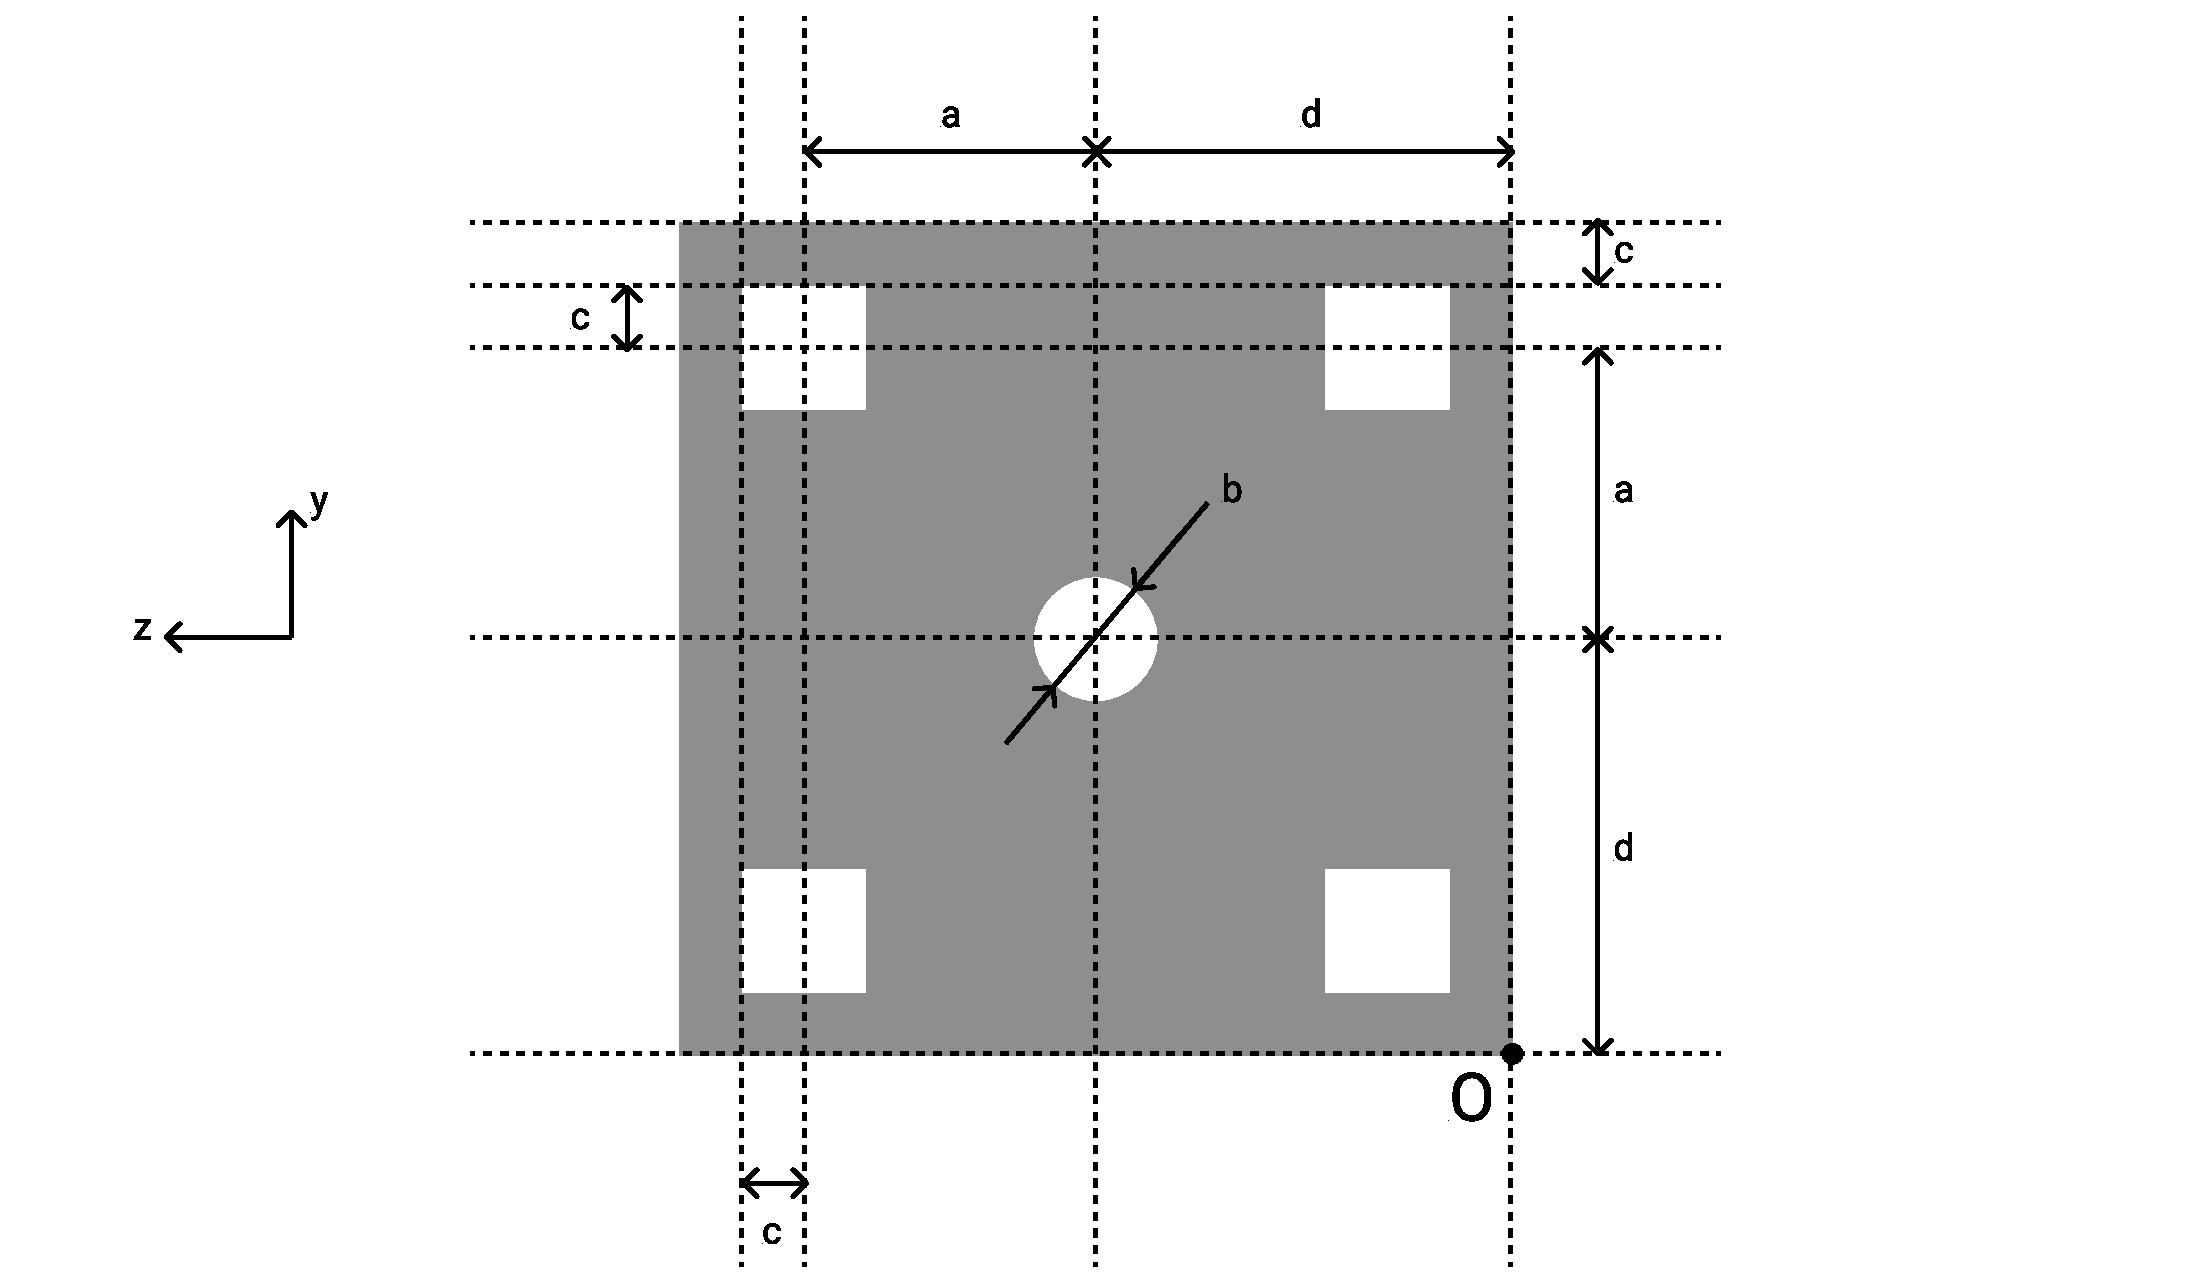
\includegraphics[width=\textwidth]{figA0024.pdf}
\end{center}

\medskip

On donne :

\begin{center}
  \begin{tabular}{|l|l|l|l|l|l|}
    \hline
    a = 80 mm & b = 15 mm & c = 8 mm & d = 96 mm \\
    \hline
  \end{tabular}
\end{center}

\medskip

\begin{enumerate}
  \item Soit $G$ le centre d'inertie de la section. Précisez sa position dans le repère $(yOz)$.
  \item Calculez le moment d'inertie $I_{Gz}$.
  \item On suppose un moment flechissant $M_{fz}$ constant appliqué à cette poutre. Ce type de poutre est-elle plus rigide qu'une poutre à section pleine? Justifiez.
\end{enumerate}

\finenonce{rdm-0024}
\finexercice


\end{document}
